\documentclass{article}
\usepackage[utf8]{inputenc}
\usepackage{graphicx} 
\usepackage[newfloat]{minted}
\usepackage{caption}
\usepackage{amsmath,amssymb,amsfonts}
\usepackage{algorithmic}
\usepackage{textcomp}
\usepackage{xcolor}
% \usepackage[
%     %backend=biber, 
%     natbib=true,
%     style=numeric,
%     sorting=none
% ]{biblatex}
% \addbibresource{bio.bib}
\usepackage{array}
\usepackage{type1cm}
\usepackage{lettrine}
\usepackage{siunitx}
\usepackage{subcaption}
\usepackage{pdfpages}
\usepackage{mwe}
\usepackage{subfiles}
\usepackage{multicol}
\usepackage{float}
\usepackage{blindtext}
\usepackage{hyperref}
\usepackage{listings}
\lstset{
    xleftmargin=0pt,        
    framexleftmargin=5pt,
    framesep=0pt,
    numbers=none,            
    frame=single,            
    breaklines=true,
    tabsize=4
}
\usepackage{xcolor}
\definecolor{LightGreen}{rgb}{0.2,0.4,0.2}
\definecolor{White}{rgb}{1,1,1}
\usepackage[export]{adjustbox}[2011/08/13]

\newenvironment{code}{\captionsetup{type=listing}}{}
\SetupFloatingEnvironment{listing}{name=Source Code}
\usepackage{subfiles}

\setlength\parindent{0pt}

\begin{document}

\definecolor{LightGray}{gray}{0.9}

\begin{titlepage}
    \centering
    \vfill
    {\bfseries\Large
        Intelligent Architecture Lab Manual\\
        \vskip2cm
        Lorenzo Pes, Zhanbo Shen \\
        l.pes@tue.nl, z.shen1@tue.nl \\
        
    
        \vskip1cm
        \today \\
    }    
    \vfill
    
\includegraphics[width=6cm]{NECS.png} \\
    \vskip2cm
    Neuromorphic Edge Computing Systems Lab \\
    \vfill
\end{titlepage}

%\maketitle
\tableofcontents

\newpage 
\section{SystemVerilog \footnotesize(for those who are new)}

{\large\textbf{SystemVerilog}} provides new features on top of Verilog. Some of you may not come across this tool before, which is fine because we will have a brief tutorial about the features that we will use in this lab and hope that will be enough to get you started. For those who are familiar with SystemVerilog, we meet you at the next section!\\

SystemVerilog is a hardware description and hardware verification language used to model, design, simulate, test and implement electronic systems. It is based on Verilog and some extentions, commonly used in the semiconductor and electronic design. If you are familiar with Verilog, you will find SystemVerilog easy to learn, if not, we also provide you a brief journey to the hardware description world.\\

\subsection{Data Types}
\begin{figure}[h]
    \centering
    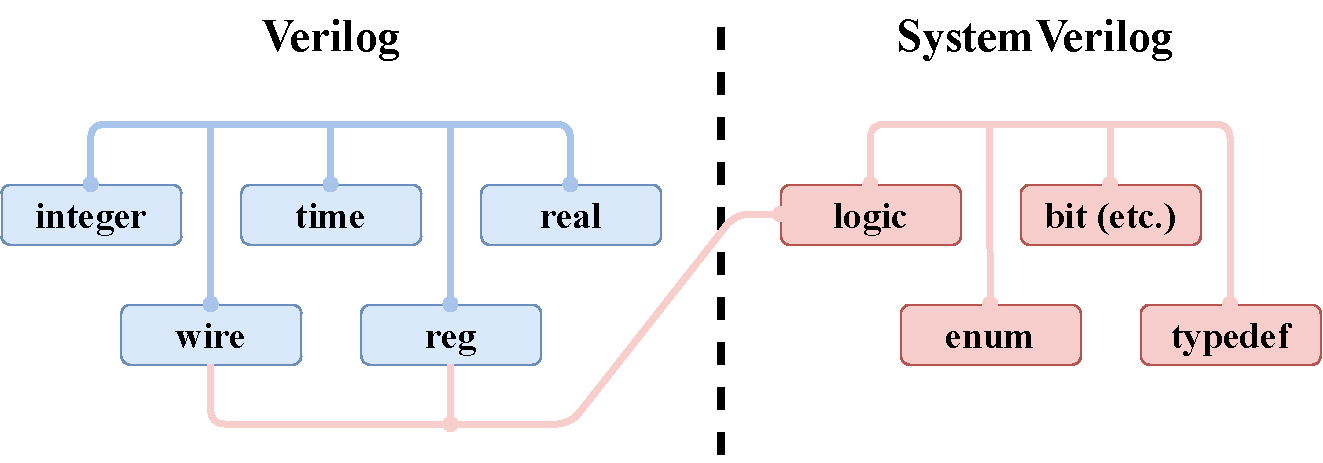
\includegraphics[width=\textwidth]{figures/DataType.pdf}
    \label{fig:DataType}
    \caption{Data Types in Verilog \& SystemVerilog}
\end{figure}
\textbf{Verilog:}
\begin{itemize}
    \item \textbf{integer:} 32-bit signed integer, only for simulation and non-synthesis purpose.
    \begin{lstlisting}[language=Verilog,frame=single,backgroundcolor=\color{White},basicstyle=\color{LightGreen},showspaces=false,showstringspaces=false]
    integer i;
    for (i=0; i<10; i=i+1) begin
        $display("i = %d", i);
    end
    \end{lstlisting}
    \item \textbf{time:} 64-bit unsigned integer, for presenting time.
    \begin{lstlisting}[language=Verilog,frame=single,backgroundcolor=\color{White},basicstyle=\color{LightGreen},showspaces=false,showstringspaces=false]
    time t_start, t_end;
    \end{lstlisting}
    \item \textbf{real:} floating number, for accurate time calculation and simulation.
    \begin{lstlisting}[language=Verilog,frame=single,backgroundcolor=\color{White},basicstyle=\color{LightGreen},showspaces=false,showstringspaces=false]
    real voltage;
    \end{lstlisting}
    \item \textbf{wire:} net type, for connecting modules and continuous assignment (combinational logic).
    \begin{lstlisting}[language=Verilog,frame=single,backgroundcolor=\color{White},basicstyle=\color{LightGreen},showspaces=false,showstringspaces=false]
    wire a, b;
    assign a = b & 1'b1;
    \end{lstlisting}
    \item \textbf{reg:} memory or register type, for storing values and sequential logic.
    \begin{lstlisting}[language=Verilog,frame=single,backgroundcolor=\color{White},basicstyle=\color{LightGreen},showspaces=false,showstringspaces=false]
    reg clk;
    always @(posedge clk) begin
        clk <= ~clk;
    end
    \end{lstlisting}
\end{itemize}

\textbf{SystemVerilog:}
\begin{itemize}
    \item \textbf{logic:} to replace wire and reg, for both combinational and sequential logic.
    \begin{lstlisting}[language=Verilog,frame=single,backgroundcolor=\color{White},basicstyle=\color{LightGreen},showspaces=false,showstringspaces=false]
        logic clk, reset;
    \end{lstlisting}

    \begin{figure}[h]
        \centering
        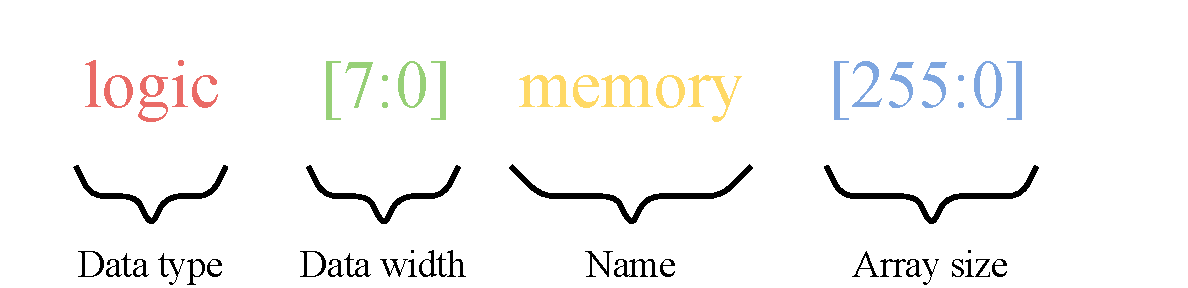
\includegraphics[width=\textwidth]{figures/array.pdf}
        \label{fig:array}
        \caption{Array in SystemVerilog}
    \end{figure}
    \item \textbf{bit (etc.):} offers more flexibility in bit manipulation.
    \begin{lstlisting}[language=Verilog,frame=single,backgroundcolor=\color{White},basicstyle=\color{LightGreen},showspaces=false,showstringspaces=false]
    bit [7:0] data;
    shortint value;
    \end{lstlisting}
    \item \textbf{enum:} enumeration type, for defining a set of named values.
    \begin{lstlisting}[language=Verilog,frame=single,backgroundcolor=\color{White},basicstyle=\color{LightGreen},showspaces=false,showstringspaces=false]
    typedef enum logic [1:0] {IDLE, BUSY, DONE} state_t;
    state_t current_state;
    \end{lstlisting}
    \item \textbf{typedef:} to define new data types.
    \begin{lstlisting}[language=Verilog,frame=single,backgroundcolor=\color{White},basicstyle=\color{LightGreen},showspaces=false,showstringspaces=false]
    typedef logic [7:0] byte_t;
    byte_t data;
    \end{lstlisting}
\end{itemize}
SystemVerilog also offers some advanced data types, such as \textbf{struct, union, array, queue}, etc. You will see them if they are used in the lab, we do not cover them here.\\

\subsection{Combinational Logic}
Combinational logic refers to circuits or logic blocks whose outputs depend entirely on their current inputs, without any form of internal storage or memory.
\begin{table}[h]
    \centering
    \begin{tabular}{|c|c|c|}
        \hline
        \textbf{Operation} & \textbf{bit-wise} & \textbf{logic-wise} \\
        \hline
        AND & \& & \&\& \\
        OR & $|$ & $||$ \\
        NOT & $\sim$ & $!$ \\
        XOR & \^{} &  \\
        XNOR & \^{}\textasciitilde &  \\
        \hline
    \end{tabular}
    \caption{Combinational Logic Operations}
\end{table}
\begin{lstlisting}[language=Verilog,frame=single,backgroundcolor=\color{White},basicstyle=\color{LightGreen},showspaces=false,showstringspaces=false]
logic [3:0] a = 4'b1010;
logic [3:0] b = 4'b1100;
logic [3:0] and_result, or_result, not_result;
logic and_z, or_z, not_z;

assign and_result = a & b; // result = 4'b1000
assign or_result = a | b; // result = 4'b1110
assign not_result = ~a; // result = 4'b0101
assign and_z = a && b; // z = 1'b1
assign or_z = a || b; // z = 1'b1
assign not_z = !a; // z = 1'b0
\end{lstlisting}

\subsection{Sequential Logic}
Sequential logic differs from combinational logic in that the output of a sequential circuit depends not only on its current inputs, but also on its past inputs or state. And sequential logic always requires a clock signal to control the timing of the circuit.

\begin{multicols}{2}
    \textbf{combinational logic:}\\

    \begin{lstlisting}[language=Verilog,frame=single,backgroundcolor=\color{White},basicstyle=\color{LightGreen},showspaces=false,showstringspaces=false]
module mux4to1 (
    input logic [3:0] data,
    input logic [1:0] sel,
    output logic out
);
    always @(*) begin
        case (sel)
            2'b00: out = data[0];
            2'b01: out = data[1];
            2'b10: out = data[2];
            2'b11: out = data[3];
        endcase
    end
endmodule
    \end{lstlisting}
    \columnbreak
    \textbf{sequential logic:}\\

    \begin{lstlisting}[language=Verilog,frame=single,backgroundcolor=\color{White},basicstyle=\color{LightGreen},showspaces=false,showstringspaces=false]
module counter (
    input logic clk, reset,
    output logic [3:0] count
);
    always @(posedge clk or posedge reset) begin
        if (reset) begin
            count <= 4'b0000;
        end else begin
            count <= count + 1;
        end
    end
endmodule
    \end{lstlisting}
\end{multicols}

\textcolor{red}{\textbf{Combinational logic}} typically describes hardware where the output depends directly on the input without clock control. Blocking assignments (=) ensure that values are updated immediately and in the proper sequence. In \textcolor{red}{\textbf{Sequential logic}}, non-blocking assignments (\textless =) reflect how registers in hardware update their values simultaneously.

\subsection{Finite State Machine (FSM)}
An FSM is a mathematical and conceptual model used to design digital logic circuits that exhibit sequential behavior. It is composed of a finite number of states, transitions between those states, and actions. An FSM can be in one of the finite number of states at any given time, and it changes from one state to another in response to input signals and timing events.

Key concepts in FSM:
\begin{itemize}
    \item \textbf{State:} Each state represents a condition or mode of the system.
    \item \textbf{Transition:} An FSM transitions from one state to another based on input signals and timing events. A transition defines under what input conditions the machine moves from one state to another.
    \item \textbf{Inputs and Outputs:} \texttt{inputs} are external signals or conditions that influence state transitions, and \texttt{outputs} are signals generated by the FSM that depend either on the current state alone (Moore machine) or on both the current state and the inputs (Mealy machine).
\end{itemize}

Components of an FSM:
\begin{itemize}
    \item State register (sequential logic): stores the current state.
    \item Next state logic (combinational logic): determines the next state based on the current state and inputs.
    \item Output logic (combinational or sequential logic): generates outputs based on the current state (with the inputs in Mealy machine).
\end{itemize}
Here is an example of a Mealy machine in SystemVerilog:
\begin{lstlisting}[language=Verilog,frame=single,backgroundcolor=\color{White},basicstyle=\color{LightGreen},showspaces=false,showstringspaces=false]
module mealy_pattern_detector (
    input  logic clk,
    input  logic rst_n,
    input  logic in_bit,      // Serial input stream
    output logic pattern_found // Output goes high for one cycle when "101" is detected
    );
    
    //---------- State Declaration ----------
    typedef enum logic [1:0] {
        IDLE  = 2'b00,
        S1    = 2'b01,
        S10   = 2'b10
    } state_t;
    
    state_t current_state, next_state;
    
    //---------- State Register (Sequential) ----------
    always_ff @(posedge clk or negedge rst_n) begin
        if (!rst_n)
        current_state <= IDLE;
        else
        current_state <= next_state;
    end
    
    //---------- Next-State Logic (Combinational) ----------
    always_comb begin
        // Default next state
        next_state = current_state;
        
        case (current_state)
        IDLE: begin
            if (in_bit == 1)
            next_state = S1;
            else
            next_state = IDLE;
        end
    
        S1: begin
            if (in_bit == 0)
            next_state = S10;  // matched "10"
            else
            next_state = S1;   // still have a '1' that might start a new pattern
        end
    
        S10: begin
            if (in_bit == 1)
            next_state = S1;  // matched "101" and the new '1' could be a start
            else
            next_state = IDLE;
        end
        endcase
    end
    
    //------------- Output Logic ---------------
    always_comb begin
        // Default output
        pattern_found = 1'b0;
    
        // Pattern is detected when transitioning through S10 with in_bit == 1
        // Because Mealy outputs depend on state + input, we check those conditions directly
        if ((current_state == S10) && (in_bit == 1))
        pattern_found = 1'b1;
    end
    
endmodule
\end{lstlisting}

This code is used to fine the input pattern "101" in a serial input stream. Following is the state diagram of the FSM to help you understand how it works.
\begin{figure}[h]
    \centering
    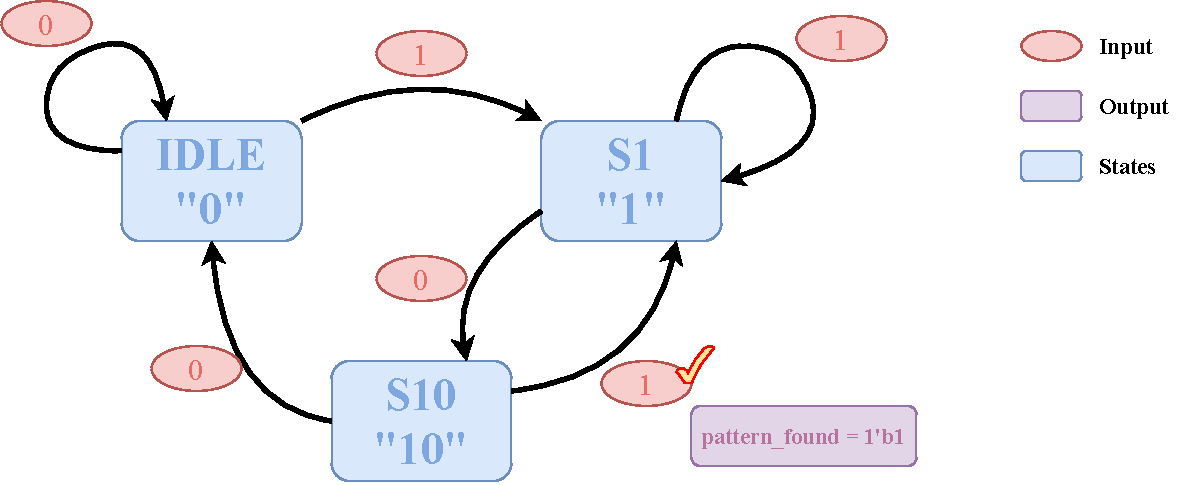
\includegraphics[width=\textwidth]{figures/state_diagram.pdf}
    \label{fig:FSM}
    \caption{State Diagram of a Mealy machine}
\end{figure}
\end{document}